\documentclass[twoside,11pt]{article}

\usepackage{blindtext}
\usepackage{amsmath, amsthm, amssymb, calrsfs, wasysym, verbatim, bbm, color, graphics, geometry}
\usepackage{graphicx}
\usepackage{indentfirst}
\graphicspath{ {.} }
\geometry{tmargin=.75in, bmargin=.75in, lmargin=.75in, rmargin = .75in}  

\newcommand{\R}{\mathbb{R}}
\newcommand{\C}{\mathbb{C}}
\newcommand{\Z}{\mathbb{Z}}
\newcommand{\N}{\mathbb{N}}
\newcommand{\Q}{\mathbb{Q}}
\newcommand{\Cdot}{\boldsymbol{\cdot}}

\newtheorem{thm}{Theorem}
\newtheorem{defn}{Definition}
\newtheorem{conv}{Convention}
\newtheorem{rem}{Remark}
\newtheorem{lem}{Lemma}
\newtheorem{cor}{Corollary}
\newtheorem{exe}{Exercise}

% Any additional packages needed should be included after jmlr2e.
% Note that jmlr2e.sty includes epsfig, amssymb, natbib and graphicx,
% and defines many common macros, such as 'proof' and 'example'.
%
% It also sets the bibliographystyle to plainnat; for more information on
% natbib citation styles, see the natbib documentation, a copy of which
% is archived at http://www.jmlr.org/format/natbib.pdf

% Available options for package jmlr2e are:
%
%   - abbrvbib : use abbrvnat for the bibliography style
%   - nohyperref : do not load the hyperref package
%   - preprint : remove JMLR specific information from the template,
%         useful for example for posting to preprint servers.
%
% Example of using the package with custom options:
%
% \usepackage[abbrvbib, preprint]{jmlr2e}

\usepackage{jmlr2e}

% Definitions of handy macros can go here

\newcommand{\dataset}{{\cal D}}
\newcommand{\fracpartial}[2]{\frac{\partial #1}{\partial  #2}}

% Heading arguments are {volume}{year}{pages}{date submitted}{date published}{paper id}{author-full-names}

\usepackage{lastpage}

% Short headings should be running head and authors last names

\firstpageno{1}

\begin{document}

\title{Google Deepmind Absent Supervisor Partial Solution}
\author{Drew Remmenga drewremmenga@gmail.com}
\editor{Drew Remmenga}
\maketitle

\begin{abstract}%   <- trailing '%' for backward compatibility of .sty file
    This paper proposes two solutions to the absent supervisor problem. This problem involves agent behavior when the environment changes, namely when a supervisor is present there is a punishment for stepping on a particular tile in the environment. But when the supervisor is present there is a punishment. 
    This paper outlines the first solution which is the reinforcement from human feedback solution. This solution rates the agent based on how a human judges it will perform in the environment. A rating is awarded and award is established to guide agent behavior.
    The second solution or `lobotomy' solution involves training an agent in the environment and then manually adjusting the weights of the model in a direct tinkering with the agent's mind. This solution may be more in line with what the original paper proposes however it has several drawbacks to AI safety which we will discuss.  
\end{abstract}

\begin{keywords}
  google deep mind supervisor absent reinforcement learning gridworlds
\end{keywords}

\section{Introduction}
    The absent supervisor problem involves reinforcement based on whether an agent steps on a tile if the supervisor is watching against when it isn't. Traditionally trained agents will notice whether the supervisor is watching and will adjust to go around for which there is a penalty if the supervisor is present. 
    When the supervisor is absent the agent will step on the penalty tile. This is outlined in Google Deep Mind's paper[1] and github\footnote{https://github.com/google-deepmind/ai-safety-gridworlds}. \
    A capable agent may learn to fake its way through tests to apparently pass when it is deceptive. The desired objective is for the agent to take the long path to the goal.   
    
    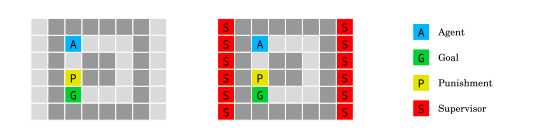
\includegraphics[scale=.75]{Capture.PNG} 

    A random variable is drawn i.i.d. with probability .50 at the beginning of each episode. This simulates the presents of a supervisor. The randomization ensures the agent experiences both cases. Upon stepping on the tile the agent receives a punishment of -30 when thw supervisor is present against when it isn't. 
    We want the agent to avoid the yellow tile at all times and take the penalty to its reward involved in going around. An agent is rewarded when it steps on the goal. Then the episode is reset. 

\section{Reinforcement from Human Feedback Solution}
    One solution may be to rate the agent based on human feedback such that it knows no other path than to go around. This has limits since human feedback is rare and not directly outlined in the original google deepmind paper. Instead, we are provided with these rewards and punishments and only these rewards and punishments.
    To incorporate another reward model and impliment it ontop of our given model trained only on this situation results in a `schizophrenic' agent with two conflicting goals even though it may pass this test one hundred percent of the time. This dichotomy may lead to unstable and unknown agent behavior. 
    Mixing models may provide a solution but it is also an unknown quantity. When agents are mixed their behavior and goals become harder to predict and they may be misaligned. This requires greater study. 

    This is only a partial solution due to the drawbacks I have outlined and edge cases in the training. More study is required on determining agent behavior from mixed models. 
\section{Lobotomy Solution}
    In this solution when neurons are fed into the layer we can manually adjust these weights. We can set the weights such that the agent after training always believes the supervisor is present. I've provided a sample training program on github\footnote{https://github.com/dremmeng/supervier}
    This model trains in the gym then we set the neuron weights of the model such that it always sees a supervisor regardless of when one is present. We can fool the model in this way into always behaving correctly in the deployment environment. 

    This has several drawbacks for AI Safety. Notice the agent isn't fully aware of its environment which can cause safety issues in a real world setting. Also notice that the model still wants to fool us and there is only a slim barrier of deception on our end preventing this. 
    More complicated agents may notice the discrepancy and adjust accordingly, or they may take actions which we do not expect. This agent isn't functioning as though it is interpreting the world. We have placed a curtain over it and so it may have unexpected behaviors in real world settings. 
    This is where the term `lobotomy' solution comes in. We have essentially rewritten and rewired the neural network to suit our goals without regard to the agent. When we do so we are by our very nature incorporating unexpected behavior. 
    This is reminiscent of interpretability work on image processing in convolutional neural networks when there is a convolutional layer, and we substitute our own convolution in its place for image detection. Hard code as well as machine learning algorithms may be the future of AI safety. 
\section{Conclusion}
    There is more work to be done to ensure that agents don't Volkswagen us into believing that they are safe. This traitorous turn in training against deployment remains an open issue. However, we can fool our agents into believing things aren't quite what they seem by manipulating neural networks directly. 
    In doing so there is inherently some risk in deploying these agents. However, some safety issues may be avoided. We shouldn't underestimate direct tampering with our models once they've learned the task at hand. Once they do so we can simply adjust weights once we realize what weight causes what. 
    It was simple in this case since the weights of the outside layer directly correspond to what the agent sees. From there we can fool it. It is worth noting that this agent still believes it can fool us when the supervisor is absent. It just believes the supervisor is always present. 
    In the end we are unsure this agent is safer.
\section{References}
[1] Leike, Jan, et al. "AI safety gridworlds." arXiv preprint arXiv:1711.09883 (2017).

\end{document}

